%Danilo
%===========================================
%   1.  Explicar que esta parte corresponde al problema directo
%   2.Presentar la fuente sísmica real simulada 
%   3.Explicar las coordenadas de la fuente
%   4.Explicar por qué z es negativo
%   5.Explicar la distancia euclidiana en R3
%============================================


\begin{frame}{Construcción del Problema Directo}

    % Usamos [c] para garantizar que todo el contenido flote exactamente en el centro vertical
    \begin{columns}[c]

        %========================================
        % COLUMNA IZQUIERDA: VISUALIZACIÓN
        %========================================
        \column{0.58\textwidth} % Le damos un poco más de ancho a la imagen

        \begin{center}
            % La imagen ahora domina este lado sin textos que compitan con ella
            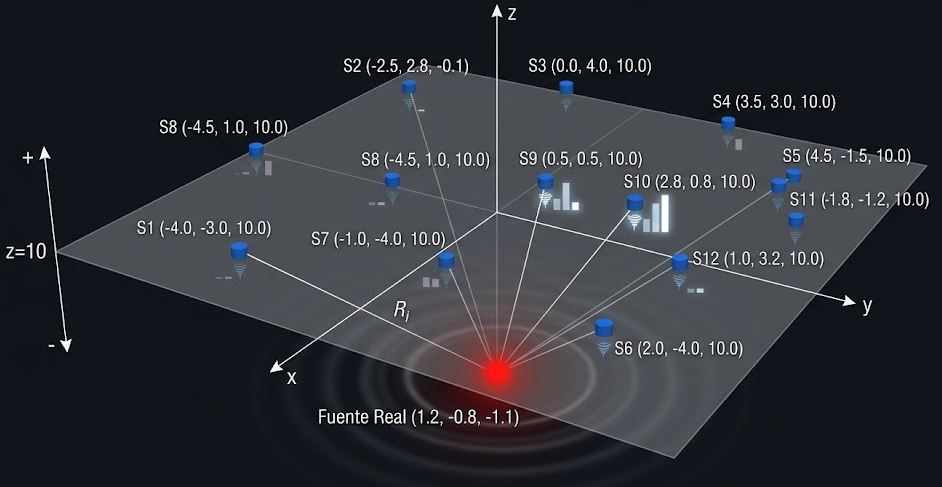
\includegraphics[width=\textwidth]{Imagenes/ProblemaDirecto3D.png}
        \end{center}

        %========================================
        % COLUMNA DERECHA: DATOS CLAVE
        %========================================
        \column{0.38\textwidth}

        %----------------------------------------
        % BLOQUE 1: ENTORNO
        %----------------------------------------
        % Convertimos el bullet point de R3 en un bloque elegante
        \begin{block}{Entorno del Modelo}
            \centering
            \vspace{0.2cm}
            Espacio tridimensional $\mathbb{R}^3$
            \vspace{0.2cm}
        \end{block}

        \vspace{0.8cm} % Un espacio grande para separar y usar bien el lienzo vacío

        %----------------------------------------
        % BLOQUE 2: PARÁMETROS REALES
        %----------------------------------------
        \begin{block}{Fuente Sísmica Real}
            \centering
            \vspace{0.2cm}
            
            \small
            \textbf{Coordenadas del Hipocentro:}
            \[
            (x_{\text{real}}, y_{\text{real}}, z_{\text{real}}) = (1.2, -0.8, -1.1)\ \text{km}
            \]
            \vspace{0.1cm}
        \end{block}

    \end{columns}

\end{frame}